%!TEX root = ../Thesis.tex
We begin this chapter with the evaluation of questionnaire and discuss the demographics and self assessment of emotions felt by the subjects while watching the movies. We then take a look at how and which features were extracted from the Eclectrocardiogram (ECG) and Electrodermal Activity (EDA) physiological data. Finally, we discuss how the extracted features were used to train a Random Forest machine learning model and a Long Term Short Memory (LSTM) neural network model for classification and prediction.

\section{Evaluation from the questionnaire}
As discussed in Section \ref{sec:procedure}, the subjects participating in the experiment were asked to fill in a questionnaire. The questionnaire constituted of two sections. The first section comprised of demographic questions like age, gender, study program, language proficiency, and movie genre preferences. The second section of the questionnaire asked the subjects to self assess their emotions after each movie. The questionnaire was inspired by Positive and Negative Affect Schedule (PANAS) scale\cite{panas_crocker:1997} to quantify the emotions the subjects felt while watching the movie. The questionnaire is attached in the appendix. In the following section, we quantify the demographics and self-assessment of emotions by the subjects.
\subsection{Demographics}
\paragraph{Gender and age} The subjects participated in the study voluntarily. There was no prerequisite for participation in the study. A total of 72 subjects participated in the study of which 52 were male and 20 were female. The subjects were 18-75 years old, with a mean age of 25.55 years and standard deviation of 8.12 years. The age distribution is shown in figure \ref{fig:age_distribution}.

\begin{figure}
    \centering
    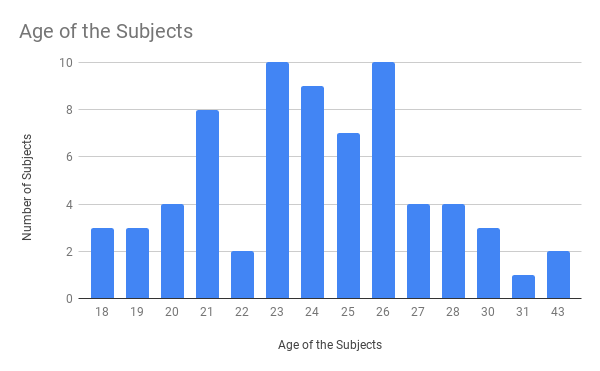
\includegraphics[width=140mm]{Figures/age_of_subjects.png}
    \caption{Age distribution of the subjects}
    \label{fig:age_distribution}
\end{figure}

\paragraph{Language proficiency} The subjects were asked to rate their English and Spanish language proficiency between unfamiliar to native. The distribution of language proficiency is shown in figure \ref{fig:english_language} and figure \ref{fig:spanish_language}. As for the native language of the subjects, 32 subjects spoke German, 19 subjects spoke Urdu, 10 subjects spoke Hindi, 2 subjects spoke Russian and one subject each for Chinese, Persian, Turkish, Vietnamese, English, Luxembourgian, Bengali, Hebrew, Fula language.

\begin{figure}
    \centering
    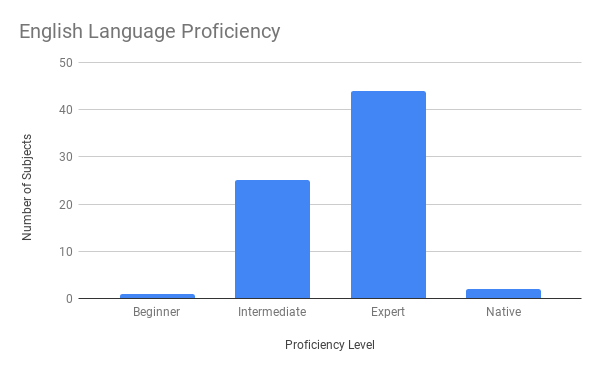
\includegraphics[width=140mm]{Figures/english_language_proficiency.png}
    \caption{English Language proficiency of the subjects.}
    \label{fig:english_language}
\end{figure}

\begin{figure}
    \centering
    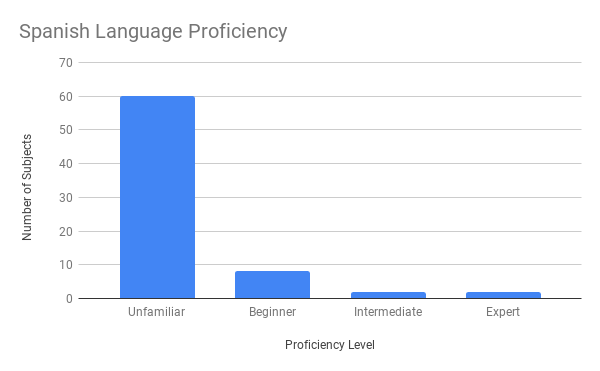
\includegraphics[width=140mm]{Figures/spanish_language_proficiency.png}
    \caption{Spanish language proficiency of the subjects.}
    \label{fig:spanish_language}
\end{figure}

\subsection{Self Assessment of Emotion}
\todo{Analyze every movie here and put the graphs in the appendix.}

\subsection{Measure of discomfort due to electrodes.}
After the session of the study ended the subjects were asked to rate how much they were distracted by the due to electrodes and if it caused them any discomfort. This was to understand if the presence of electrodes may have cause some variation in data compared to a wearable device. From the assessment made by the subjects we found out that the presence of electrodes caused no to little discomfort among the subjects. The ratings of the users are analyzed in the figure \ref{fig:discomfort}.

\begin{figure}
    \centering
    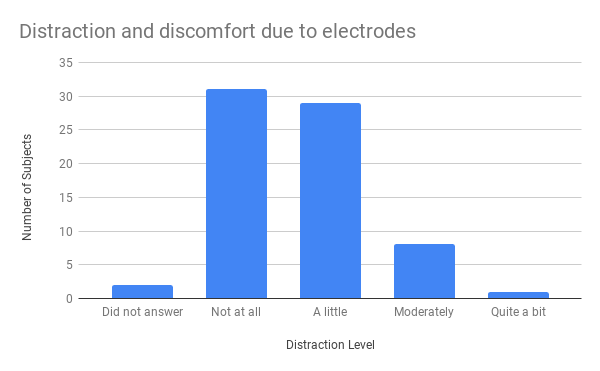
\includegraphics[width=140mm]{Figures/distraction_and_discomfort.png}
    \caption{Subject ratings of discomfort caused by electrodes.}
    \label{fig:discomfort}
\end{figure}

\subsection{Remarks}
There is an additional set of data that was included to the physiological data of the 72 subjects for this study. We took into consideration the data that we collected over the course of four months while we perfected the study procedure. We only selected the data whose signals had considerably low artifacts which could be removed by the technique described in section \ref{sec:preprocessing}. Thus physiological data of 17 subjects were taken into consideration. 
\paragraph{}However, there is no demographic or emotional self-assessment questionnaire available for this data set. A verbal consent was taken for using their data pseudo-anonymously for the study. The dataset taken into account for this study is summarized in table \ref{tab:ecg_data_set} for Electrocardiogram (ECG) data and table \ref{tab:eda_data_set} for Electrodermal Activity (EDA) data. The data collected before the questionnaire was introduced is termed 'old' and the data collected after the introduction of the questionnaire is termed 'new' in the table \ref{tab:eda_data_set}.


\begin{center}
\begin{tabular}{ |c|c|c|c| }
\hline
Movie & Old & New & Total \\
\hline
\hline
3 Versos & 11 & 33 & 44 \\
\hline
Alexia & 17 & 41 & 58 \\
\hline
Go Bag & 14 & 38 & 52 \\
\hline
The Lie Detector & 16 & 46 & 62 \\
\hline
The Last Three Minutes & 4 & 36 & 40 \\
\hline
I Miss You & 17 & 50 & 67 \\
\hline
The Most Beautiful Thing & 10 & 46 & 62 \\
\hline
\textbf{Total} & \textbf{89} & \textbf{290} & \textbf{379} \\
\hline
\end{tabular}
\captionof{table}{ECG Dataset}
\label{tab:ecg_data_set}
\end{center}

\begin{center}
\begin{tabular}{ |c|c|c|c| }
\hline
Movie & Old & New & Total \\
\hline
\hline
3 Versos & 10 & 32 & 42 \\
\hline
Alexia & 9 & 44 & 53 \\
\hline
Go Bag & 11 & 40 & 51 \\
\hline
The Lie Detector & 14 & 48 & 62 \\
\hline
The Last Three Minutes & 4 & 37 & 41 \\
\hline
I Miss You & 10 & 50 & 60 \\
\hline
The Most Beautiful Thing & 3 & 45 & 48 \\
\hline
\textbf{Total} & \textbf{61} & \textbf{296} & \textbf{357} \\
\hline
\end{tabular}
\captionof{table}{EDA Dataset}
\label{tab:eda_data_set}
\end{center}

\section{Pre-processing of Data}
\label{sec:preprocessing}
\subsection{Electrocardiogram (ECG)}
\label{sec:ecg_feature_extraction}
The Electrocardiogram is sensed by three AgCl electrodes. The Electrocardiogram (ECG) from the BITalino's ECG sensor is obtained by the measurement of voltage between two electrodes across which a low current is applied. The third electrode acts as a voltage reference. The bandwidth of BITalino's ECG sensor is 0.5-40Hz, in this range, the accuracy is guaranteed. The value sampled, \textbf{ADC}, from the BITalino is a 10-bit signal value, \textbf{n}. we use sampling frequency, \textbf{f$_{s}$} at 100Hz, 100 samples are recorded every second. The operating voltage, \textbf{V$_{CC}$}, of the ECG sensor, is 3.3V. The gain, \textbf{G$_{ECG}$} of the sensor is 1100. Thus the raw data obtained from the BITalino device over the Bluetooth can be converted to ECG value in milli-volts using the transfer function described by the equation \ref{eq:ecg}. The range of the ECG sensor is $\pm$1.5mV.

\begin{equation}
\label{eq:ecg}
    ECG(mV) = \frac{\big(\frac{ADC}{2^n} - \frac{1}{2})\times V_{cc}} {G_{ECG}}\times1000
\end{equation}

\subsubsection{Filtering} The lack of filter on at the hardware level on the MCU \cite{noauthor_faq_nodate} of the BITalino resulted in some of the ECG signals obtained from transfer having artifacts. Thus there was further need for filtering the signals to eliminate the transient noise which occurs due to movements by the subject during the recording. We filtered the signal using bandpass FIR filter with cut-off frequency between 3-40Hz similar to the approach used by \citeauthor{canento_review_nodate} \cite{canento_review_nodate}. We then used Hamilton segmenter \cite{hamilton_open_2002} to detect the correct R-peaks. The first two graphs in the figure \ref{fig:ecg_filtering} visualizes filtering of ECG signal of one of the subjects for 17 seconds segment of \textit{3 versos} movie.

\begin{figure}
    \centering
    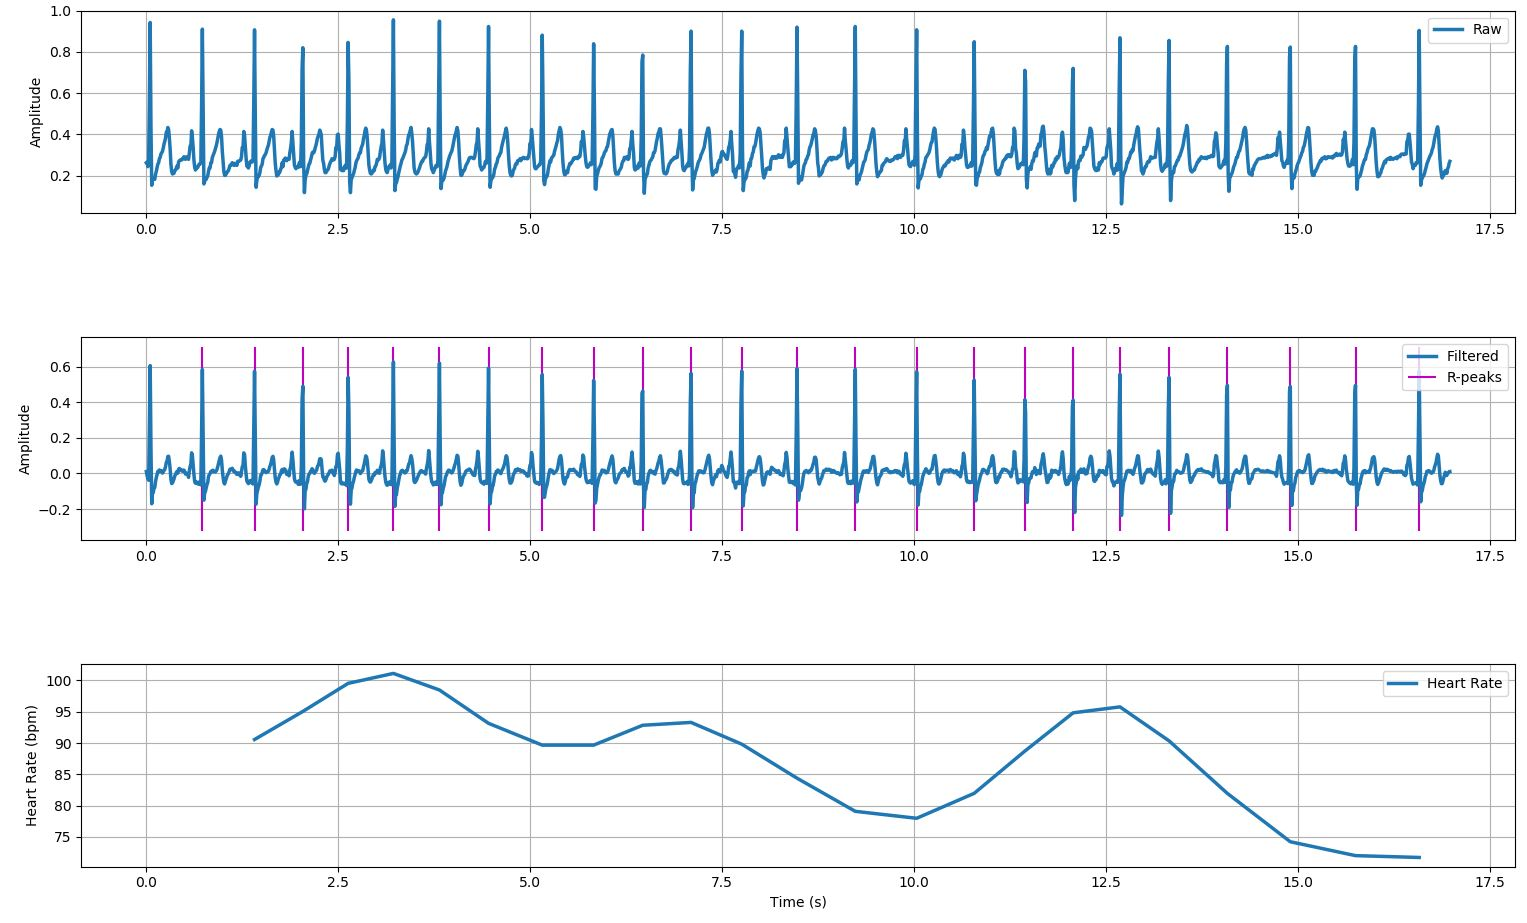
\includegraphics[width=150mm]{ecg_raw_filtered.JPG}
    \caption{Filtering and Heart Rate Variation (HRV) of ECG Signal}
    \label{fig:ecg_filtering}
\end{figure}

\subsubsection{Feature Extraction} 
\label{sec:ecg_fet_ext}
\paragraph{Heart Rate Variability (HRV)} R-R intervals are obtained by measuring the distance between two consecutive R-R peaks. A statistical artifact detection was performed on the R-R intervals, to remove the R-R intervals that differed more than 25\% from the preceding R-R interval. Next, physiological artifact detection was performed to remove the R-R intervals that were less than 0.6 seconds or more than 1.3 seconds \cite{noauthor_normal_2018}. Then the Heart Rate Variability (HRV) is calculated from the R-R interval as we discussed in section \ref{sec:rrinterval}. The bottom graph in figure \ref{fig:ecg_filtering} visualizes the filtering of the ECG signal of one of the subjects for 17 seconds segment of \textit{3 versos} movie.

\paragraph{Frequency Components} Since the Low Frequency (LF) and High Frequency (HF) have been attributed to be influenced by the activity in Parasympathetic Nervous System (PNS) and Sympathetic Nervous System (SNS) \cite{noauthor_heart_1996} \cite{berntson_gary:1997}. We extracted the frequencies of the Low Frequency (LF) between 0.04-0.15Hz and High Frequency (HF) between 0.15-0.40Hz. Furthermore, to see if there exists co-relation between other frequencies and PNS/SNS we also extracted Very Low Frequency (VLF) between 0.0033-0.05Hz and Very High Frequency (VHF) between 0.4-0.5Hz. We also computed LF/HF, LF/P, and HF/P ratios. In addition to that LFn was computed with the equation \ref{eq:lfn} and HFn with equation \ref{eq:hfn}. 

\paragraph{Miscellaneous Features} In the recent paper published by \citeauthor{zhao_emotion_2016}, the authors found that there is a significant correlation between the emotions felt by the subjects and some of the frequency domain features discussed above, time domain features, and non-linear features. Thus, we extracted the Standard Deviation of NN Intervals (sdNN), the Detrended fluctuation analysis (DFA), the pNN50 \cite{pend1995},  the Root Mean Square of Successive Differences (RMSSD), the pNN20, the Correlation\_Dimension, and the Sample Entropy. 

\begin{equation}
\label{eq:lfn}
    LFn = \frac{LF}{\big(LF + HF)}
\end{equation}

\begin{equation}
\label{eq:hfn}
    HFn = \frac{HF}{\big(LF + HF)}
\end{equation}

\subsection{Electrodermal Activity (EDA)}
\label{sec:eda_feature_extraction}
The Electrodermal Activity (EDA) is sensed by two AgCl electrodes. The Electrodermal Activity (EDA) from the BITalino's EDA sensor is obtained by measurement of voltage between two electrodes across which a low current is applied. The bandwidth of BITalino's EDA sensor is 0-2.8Hz, in this range the accuracy is guaranteed.  The value sampled, \textbf{ADC}, from the BITalino is a 10-bit signal value, \textbf{n}. Since we use sampling frequency, \textbf{f$_{s}$} at 100Hz, 100 samples are recorded every second. The operating voltage, \textbf{V$_{CC}$}, of the EDA sensor, is 3.3V. Thus the raw data obtained from the BITalino device over the Bluetooth can be converted to EDA value in mue-Siemens using the transfer function described by the equation \ref{eq:eda}. The range of the EDA sensor is 0-25$\mu$S. 


\begin{equation}
\label{eq:eda}
    EDA(\mu S) = \frac{\big(\frac{ADC}{2^n}) \times V_{cc}}{0.132}
\end{equation}

\subsubsection{Filtering} The EDA values were obtained from the transfer function in equation \ref{eq:eda}. After visualizing the signal we observed some artifacts the EDA signal. This was evident as BITalino does not have any filter at the hardware level on the MCU \cite{noauthor_faq_nodate}. There was a transient noise in some parts of the signal which occurs due to movements by subjects during the recording. In some of the signals, we also observed a static noise. This was probably because the manual denoising of the sensor as discussed in section \ref{sec:denoising}, did not effectively remove the static noise. We used the \textit{neurokit} \footnote{https://github.com/neuropsychology/NeuroKit.py} package to filter the EDA signals. We used Butterworth Lowpass Filter from the package for filtering our signal. We set the cut-off frequency of 5Hz with order N=4 to decrease the noise. The figure \ref{fig:eda_filtering_} visualizes the filtering of the EDA signal of one of the subjects \textit{3 Versos} movie.

\begin{figure}
    \centering
    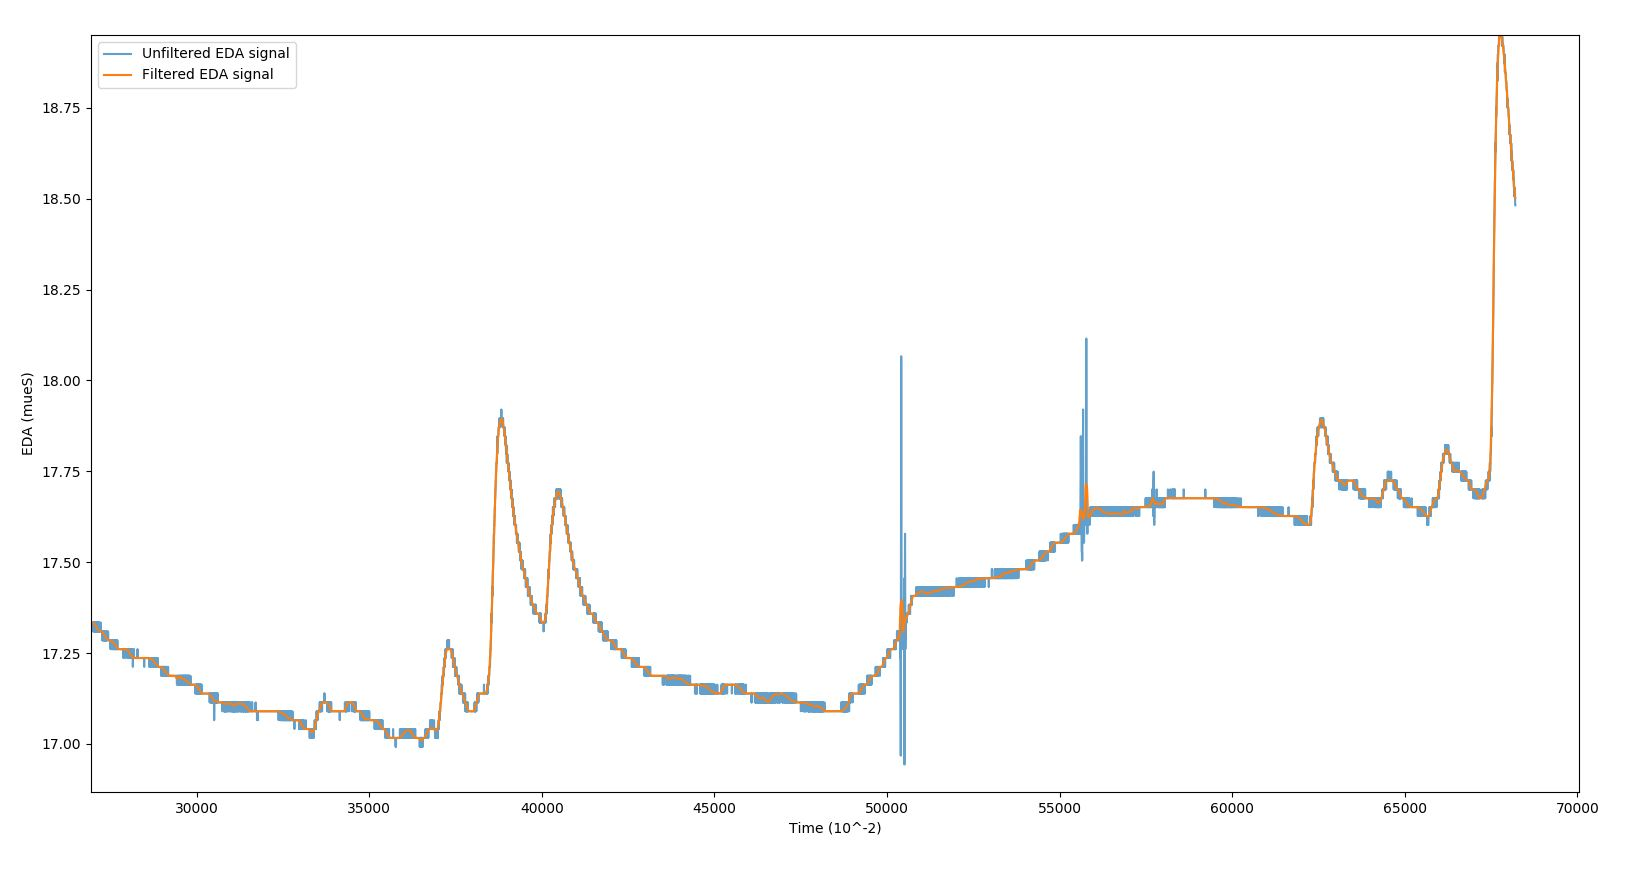
\includegraphics[width=150mm]{eda_filtering.JPG}
    \caption{Filtering of EDA Signal}
    \label{fig:eda_filtering_}
\end{figure}

\subsection{Scaling}
\label{sec:eda_scaling}
We observed that the EDA data collected had a lot of variation from one subject to another. Due to subjects physiology and state of mind during the study, some subjects had high EDA while others had low EDA. Also, some subjects had a larger variation in EDA over the period of study than others. To normalize the EDA data, we applied scaling on the filtered data. The reason for applying scaling after filtering was to eliminate outliers and artifacts influencing scaling of the EDA data. The scaling would enhance the peaks for the EDA data with low variations. As discussed in section \ref{sec:eda_sensor} the range of EDA sensor is between 0-25$\mu$S. So maintain that range for feature selection we decided to scale the data between 0-25.
\paragraph{Remarks} Scaling of ECG data was not required since we perform feature extraction in the frequency domain.

\subsubsection{Feature Extraction}
\label{sec:eda_fet_ext}
\paragraph{Phasic Component} As we discussed in section \ref{sec:tonic_phasic_eda}, EDA can be described as the sum of three components: the tonic component, the phasic component, and an additive Gaussian noise due to measurement errors and artifacts. For our analysis, we required the phasic component, which is a fast-moving component influenced by external stimuli. We thus used cvxEDA algorithm proposed by \citeauthor{greco_cvxeda:_2016} The algorithm is based on Bayesian statistics, mathematical convex optimization and sparsity. It has been shown to accurately decomposes the Electrodermal Activity (EDA) signal into phasic and tonic components \cite{greco_cvxeda:_2016}. The figure \ref{fig:phasic_tonic_visualization} visualizes the filtered Electrodermal Activity (EDA) signal, and the phasic and tonic component extracted from it. 

\begin{figure}
    \centering
    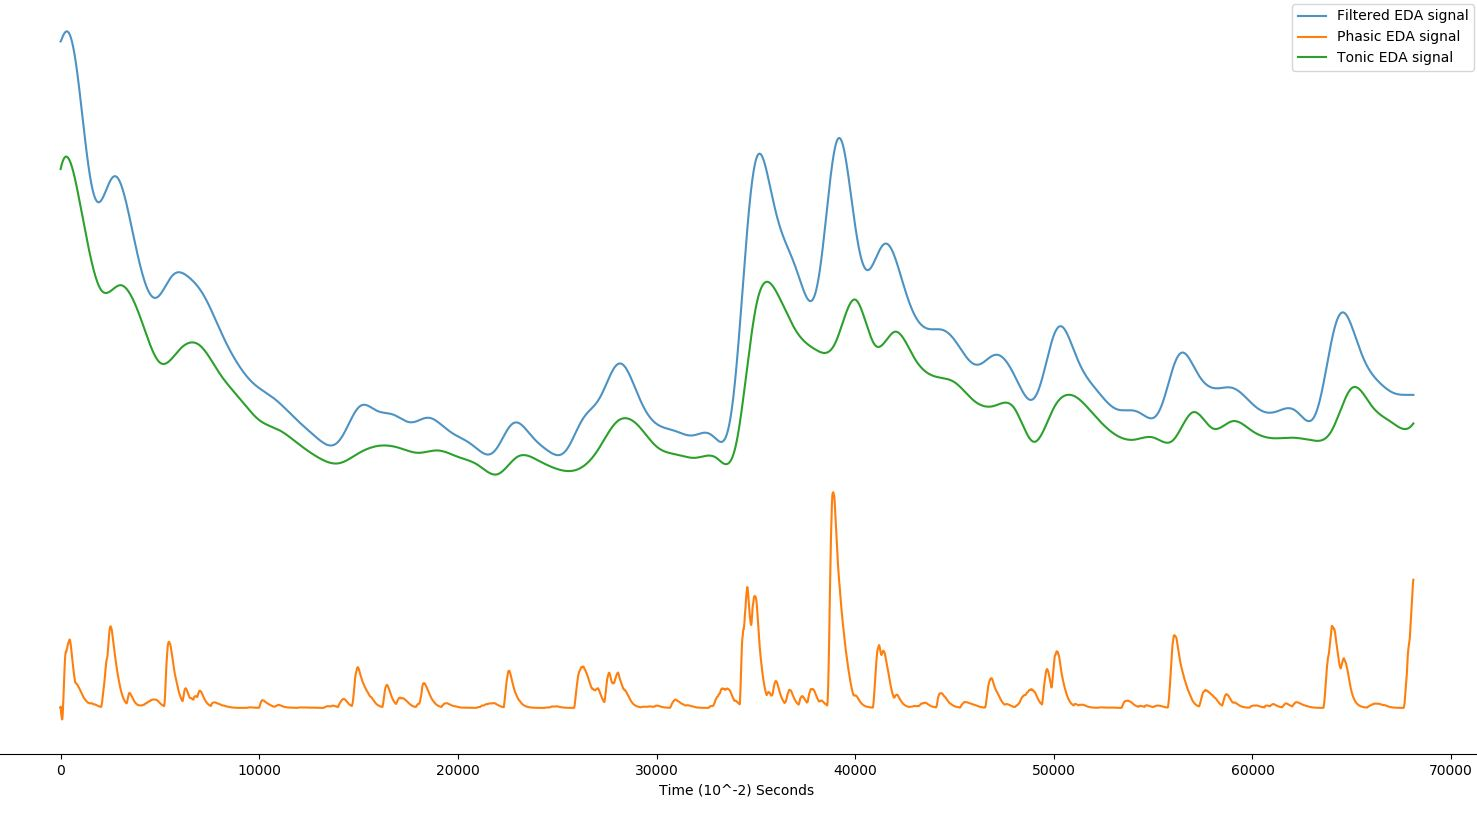
\includegraphics[width=140mm]{phasic_tonic_eda_visualization.JPG}
    \caption{Visualization of Phasic and Tonic EDA components}
    \label{fig:phasic_tonic_visualization}
\end{figure}


\paragraph{EDA Onsets} As we have discussed in section \ref{sec:quantify_eda}, given the Electrodermal Activity (EDA) in time domain. The Onset can be defined as the time at which the external stimuli was induced on to the subject. This is resonated by a drastic increase in the Electrodermal Activity (EDA) level and subsequently recovering after peaking in the time window of 3-5 seconds this has been visualized in figure \ref{fig:eda_graph} in section \ref{sec:quantify_eda} of chapter \ref{chapter:terminology}.

\paragraph{} We utilized the method proposed by \citeauthor{kim_emotion_2004} in their research done in 2004. The method detects the occurrence of EDA onset. In the first step, differentiation and subsequent convolution with the Bartlett window on the filtered EDA signal. Unlike proposed by the author, we did not downsample the signal for smoothing of the signal using the Bartlett window. We maintained the sample rate of 100Hz and window size of 100, since the result would be same as sampling rate of 20Hz and window size of 20. After convolution of the signal, the occurrence of the onset is detected by finding two consecutive zero-crossings, from negative to positive and positive to negative. The amplitude of the EDA is obtained by the maximum value between the two zero-crossing. The mean value of the amplitudes and the time point of the highest amplitude between the two zero-crossings is extracted as peak index and EDA onset respectively. We used the wrapper function provided by \textit{neurokit} python package to extract the Electrodermal Activity (EDA) features. The EDA onsets extracted using this algorithm are visualized in figure \ref{fig:eda_onsets}.

\begin{figure}
    \centering
    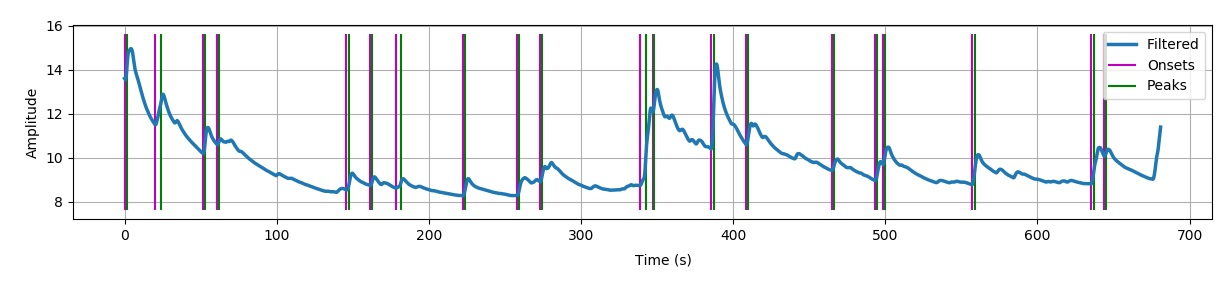
\includegraphics[width=140mm]{eda_onset.JPG}
    \caption{Visualization of EDA onsets.}
    \label{fig:eda_onsets}
\end{figure}

\section{Analysis and Results}
\subsection{Electrocardiogram (ECG) Analysis and Results}
\subsubsection{Approach}
\paragraph{Random Forest} Random forest \cite{breiman2001random} is a popular machine learning method based on decision trees. It is used for classification, regression or survival trees. In each split within the tree, the impurity reduction is maximized. This reduction is measured by the Gini index for classification, the sum of squares for regression and by the log-rank statistics or Harrell's C-index for survival outcomes \cite{wright_splitting_2019}. Random forest is part of ensemble methods. The ensemble methods combine the predictions of several base estimators built with a given learning algorithm to improve robustness over a single base estimator.
\paragraph{} In random forests each tree in the ensemble is built from a sample from the training dataset. When splitting a node during construction the best split is a random subset of the features instead of the best split among the features. As a result of the bias of the forest increases as compared to the bias of non-random trees. But due to averaging, the variance of the random forests also decreases. This compensates for the increase in the bias, thus yielding a better model.

\subsubsection{Analysis}
\paragraph{Data Preparation}  We performed the filtering, scaling and feature extraction as discussed in the section \ref{sec:ecg_feature_extraction}. No further processing was done on the extracted features.

\paragraph{Implementation} We implemented random forest classifier to classify the ECG features based on the movies. Since not all features we extracted might be helpful for our analysis. We wanted to understand which features are significant for the classification of the movies. Therefore, we ran a feature selection algorithm on top of the random forest. We used the recursive feature elimination and cross-validated (RFECV) selection algorithm to select the significant features.

\paragraph{} In our analysis, we selected the features roughly based on the paper by \citeauthor{zhao_emotion_2016} to classify emotions. These features were then fed into the RFECV. The RFECV uses random forest algorithm to select the best features. Thus we determine the subset of our selected features which are significant in increasing the accuracy of prediction.

\todo{Correct the configuration of the machine}
\paragraph{} We ran our implementation on a 96 core machine with a clock speed of 2.6GHz and 512GB of RAM. In all our evaluation, the ECG data for all the movies mentioned in table \ref{tab:shortlist_movies} were taken into consideration. the dataset was split as 90\% of data for training and 10\% for testing. Since there was a large variance between the samples of the dataset we decided to run our implementation 10 times with a different training and testing data each time to avoid false-positive results. The summary of which is discussed in the section \ref{sec:ecg_analysis_results}. In a total of 379 data samples in the data set, 341 samples were used for training and 38 samples were used for testing. 

\subsubsection{Results}
\label{sec:ecg_analysis_results}
\paragraph{Features set roughly based on \citeauthor{zhao_emotion_2016}} Here we took into consideration the pNN50, Standard Deviation of NN Intervals (sdNN), the LF/HF ratio, the Sample Entropy (SamEnt), the DFA$_{1}$ and the DFA$_{2}$ features extracted from the ECG dataset. The results are summarized in the table \ref{tab:ecg_rf_results}. The 'True' notation means that the feature was selected in the training phase to determine the accuracy of the model and 'Fales' notation means that the feature was not selected. The overview of 10 evaluations show that 7 times of 10, all the features were selected for the training of random forest and yielded an accuracy of 39\%. We note that since 7 movies are under consideration, the probability of movie being recognized by chance is 14\%. Thus, we conclude that there exists some co-relation between the subject's ECG data and their viewing activity as discussed under our goal for the thesis in chapter \ref{chapter:motivation}. However, the results can be further improved. We discuss our suggestions on improving the results in the section \ref{sec:future_work}. We also tested the other features we extracted. None of them yielded any significant improvement in our results.

\begin{center}
\resizebox{\textwidth}{!}{
\begin{tabular}{ |c|c|c|c|c|c|c|c| }
\hline
&\multicolumn{6}{c}{Features of ECG}& \\
    \cline{2-7}
Evaluation & sdNN & pNN50 & LF/HF & DFA$_{1}$ & DFA$_{2}$ & SamEnt & Accuracy \\
\hline
\hline
1 & \textbf{True} & False & \textbf{True} & \textbf{True} & \textbf{True} & \textbf{True} & 31\% \\
\hline
2 & \textbf{True} & \textbf{True} & \textbf{True} & \textbf{True} & \textbf{True} & \textbf{True} & 38\% \\
\hline
3 & \textbf{True} & False & \textbf{True} & \textbf{True} & False & \textbf{True} & 24\% \\
\hline
4 & \textbf{True} & \textbf{True} & \textbf{True} & \textbf{True} & \textbf{True} & \textbf{True} & 46\% \\
\hline
5 & \textbf{True} & \textbf{True} & \textbf{True} & \textbf{True} & \textbf{True} & \textbf{True} & 37\% \\
\hline
6 & \textbf{True} & False & \textbf{True} & False & False & \textbf{True} & 35\% \\
\hline
7 & \textbf{True} & \textbf{True} & \textbf{True} & \textbf{True} & \textbf{True} & \textbf{True} & 43\% \\
\hline
8 & \textbf{True} & \textbf{True} & \textbf{True} & \textbf{True} & \textbf{True} & \textbf{True} & 37\% \\
\hline
9 & \textbf{True} & \textbf{True} & \textbf{True} & \textbf{True} & \textbf{True} & \textbf{True} & 35\% \\
\hline
10 & \textbf{True} & \textbf{True} & \textbf{True} & \textbf{True} & \textbf{True} & \textbf{True} & 36\% \\
\hline
\end{tabular}}
\captionof{table}{Analysis of results of LSTM model on physiological dataset on the movies.}
\label{tab:ecg_rf_results}
\end{center}

\subsection{Electrodermal Activity (EDA) Analysis and Results}
\label{sec:eda_ana_results}
\subsubsection{Approach}
\paragraph{LSTM} Neural networks are powerful tool for pattern classification based on deep learning techniques. Long Short Term Memory (LSTM) is one of the powerful recurrent neural networks used for time-series classification and pattern recognition. The earliest models of LSTM used concept of self-circulation to generate path for long-term continuous flow of gradients. \cite{long_short_hochreiter}. The important extensons added to the LSTM was to make the weight of self-looping context-sensitive rather than fixed. This helps in overcoming the problem caused by a traditional recurring neural networks using excessive number of layers in time-series data. Correlations between time-series data, both long and short can be handled by using a hidden layer as a memory unit in a LSTM network. In LSTM a gated structure dictates the weight of the self-loop, and the accumulated time scale can be dynamically changed.

\begin{figure}
    \centering
    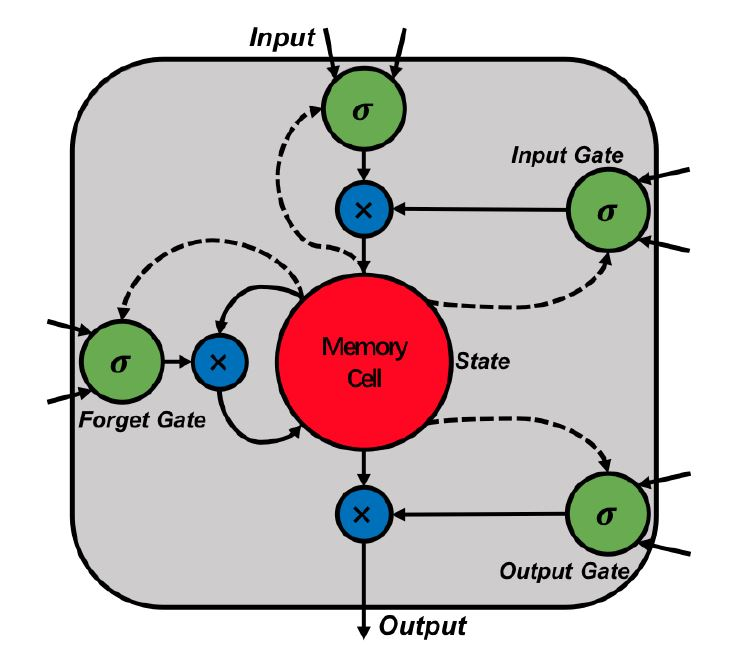
\includegraphics[width=140mm]{lstm.JPG}
    \caption{Structure of the LSTM}
    \label{fig:lstm_structure}
\end{figure}
 Neural networks are a powerful tool for pattern classification based on deep learning techniques. Long Short Term Memory (LSTM) is one of the powerful recurrent neural networks used for time-series classification and pattern recognition. The earliest models of LSTM used the concept of self-circulation to generate a path for the long-term continuous flow of gradients. \cite{long_short_hochreiter}. The important extensions added to the LSTM was to make the weight of self-looping context-sensitive rather than fixed. This helps in overcoming the problem caused by a traditional recurring neural network using an excessive number of layers in time-series data. Correlations between time-series data, both long and short can be handled by using a hidden layer as a memory unit in an LSTM network. In LSTM a gated structure dictates the weight of the self-loop, and the accumulated time scale can be dynamically changed.
 
\paragraph{LSTM Structure} The most widely used LSTM model is visualized in figure \ref{fig:lstm_structure}. In this model \textit{input gate} controls if or not value can be added to the \textit{memory cell}. The \textit{state} unit can be linearly self-looping, and it's weight is controlled by \textit{forget gate}. The \textit{output} of the cell is controlled by \textit{output gate}. All gate units can perform a sigmoid nonlinear transformation, and the input unit can have any compression non-linearity. The LSTM network can be defined by the following series of the equation:

\begin{equation}
\label{eq:lstm_1}
    i_{t} = \sigma \small(W^iH + b^i)
\end{equation}
\begin{equation}
\label{eq:lstm_2}
    f_{t} = \sigma \small(W^fH + b^f)
\end{equation}
\begin{equation}
\label{eq:lstm_3}
    o_{t} = \sigma \small(W^oH + b^o)
\end{equation}
\begin{equation}
\label{eq:lstm_4}
    c_{t} = \sigma \small(W^cH + b^c)
\end{equation}
\begin{equation}
\label{eq:lstm_5}
    m_{t} = f_{t}\cdot m_{t-1} + i_{t}\cdot c_{t}
\end{equation}
\begin{equation}
\label{eq:lstm_6}
    h_{t} = tanh\small(o_{t}\cdot m_{t})
\end{equation}


\paragraph{} In the equations \textit{i$_{t}$}, \textit{f$_{t}$}, \textit{o$_{t}$}, \textit{c$_{t}$} denote enter threshold values, forget gate values, output gate values, and new states of memory cell. $\sigma$ is a sigmoid function, and \textit{W$_{i}$}, \textit{W$_{f}$}, \textit{W$_{o}$}, and \textit{W$_{c}$} are weight matrix. \textit{b$_{i}$}, \textit{b$_{f}$}, \textit{b$_{o}$}, and \textit{b$_{c}$} are offset terms. \textit{H} is the concatenation of the new input \textit{x$_{t}$} and the previous hidden vector \textit{h$_{t-1}$}. \textit{m$_{t}$} is the final state of the memory cell, and \textit{h$_{t}$} is the \textit{output} of memory unity.

\paragraph{} In the following sections, we will discuss the two implementations of LSTM we did to analyze our data. To reiterate on we are trying to train the model to predict the movies based on the test data. We will describe the data prepared for training, the hyperparameters and implementation of LSTM, and the results.

\subsubsection{Base LSTM Model}
\label{sec:lstm_base_model}
\paragraph{Data Preparation}

We performed the filtering, scaling and feature extraction as discussed in the section \ref{sec:eda_feature_extraction} to get the phasic EDA for all subjects and movies. We analyzed this model for the phasic EDA, a time-series. We evaluated our model different combination and group size of movies. There were two reasons for this. Firstly, in our initial analysis, we found that the accuracy of the model was very high only to realize that the different lengths of the movie were allowing our model to predict the movie easily. Thus, we then altered the data fed to our model. We considered the smallest length of the sample in the data under scrutiny for the group of the movies and pruned the beginning part of all other samples to match the sample with the smallest length. Since the smallest movie in our dataset is of only 120 seconds and the longest movie is of 823 seconds, it was important for us that analysis was performed properly on the available dataset. Secondly, with different group sizes, we wanted to understand if our model is scalable. Thus, we tested our model for a combination of two, four and six movies. 

\paragraph{Architecture} The base model comprises of a single hidden layer followed by a dropout layer intended to reduce overfitting of the model to the training data. Two dense fully connected layers are used to interpret the features extracted by the LSTM hidden layer followed by a softmax logistic regression layer. The dense layer employ rectified linear units (ReLUs) to compute the feature maps. A number of recurrent dense layers can be employed to improve the accuracy of the model. \citeauthor{karpathy_visualizing_2015} in their paper showed that depth of at least two recurrent layers is beneficial when processing of sequential data. Due to lack of time, we limited our analysis to two recurrent dense layers as the increase in the number of layers would significantly increase the processing time. 

\paragraph{Hyperparameters} We used the Keras \cite{keras} package to do our analysis. Default parameters provide by Keras were used with some changes. In the LSTM layer, we used the default tanh activation function. Following which we use a dropout layer with a value of 0.5 to reduce overfitting of our model. As discussed above we used rectified linear units (ReLU) as activation for the dense layer. We used the Adam for the gradient optimization algorithm \cite{kingma_adam:_2014} and categorical cross entropy loss function as it is a multi-class classification problem. 

\todo{Correct the machine configuration}
\paragraph{Model implementation and training} We ran our model to train and test the data set on a 96 core machine with a clock speed of 2.6GHz and 512GB of RAM. We ran the training data with different size grouping of the movies. The sampling rate of physiological data used in the dataset was maintained at the sampling rate of 100Hz. Due to time limitation, not all the combinations were tested. We randomly selected the movies for the grouping. We cannot judge the accuracy of the model by a single evaluation. The reason for this is that the neural networks are stochastic. Meaning, a different specific model will result when training the model with the same configuration and with different training and test data. We determine the accuracy of our model based on an average of 5 evaluation on a model trained for each of the groupings of the movies. In all our evaluation, the dataset was split as 90\% of data for training and 10\% for testing.

\paragraph{} Two other important parameters that greatly influence the accuracy of the model are the batch size and the epoch. The batch size, \textbf{B$_{s}$} is the number of samples that will be passed through to the network at one time. The larger the batch size the quicker the model will be trained however with a trade-off is degradation of the quality of the model. Thus we tested our model with different batch sizes. Epoch is one single pass of the data through to the network. A smaller number of epochs, \textbf{E$_{s}$} may result in underfitting of the data while a larger number of epochs may result in overfitting of the data. Thus we tested our model for different epochs size.

\todo{Results are not correct. fill in the table and discuss the result.}
\paragraph{Results} The results are analyzed below.
\begin{center}
\resizebox{\textwidth}{!}{
\begin{tabular}{ |c|c|c|c|c|c|c| }
\hline
&&&\multicolumn{3}{c}{Accuracy (average of 5 evaluation)}& \\
    \cline{4-6}
Movie Group & Sample  & Number of & \textbf{E$_{s}$}=10 & \textbf{E$_{s}$}=100 & \textbf{E$_{s}$}=100 & Probablity of \\
& size &samples (Train/Test) & \textbf{B$_{s}$}=10 &  \textbf{B$_{s}$}=10 &  \textbf{B$_{s}$}=100 & Chance \\
\hline
\hline
Alexia \& Go Bag & 40000 & 92/11 & 54\% & \textbf{61\%} & 52\% & 50\%\\
\hline
Alexia \& Go Bag & 40000 & 135/16  & 41\% & \textbf{41\%} & 35\% & 33\% \\
\& TMBT & & &  & & & \\
\hline
Alexia \& Go Bag & 40000 & 173/20 & 26\% & \textbf{38\%} & 25\% & 25\% \\
\& TV \& TMBT & & & & && \\
\hline
Alexia \& Go Bag & 32000 & 228/26 & \% & \% & \% & 20\% \\
\& TV \& TMBT \& IMY & & & & & &\\
\hline
Alexia \& Go Bag \& TV & 24000 & 257/29 & \textbf{22\%} & \% & \% & 16\%  \\
\& TLTM \& TMBT \& IMY & & & & & &\\
\hline
Alexia \& Go Bag \& TLD & 12000 & 317/36 & 18\% & \textbf{21\%} & 16\% & 14\%  \\
\& TLTM \& TMBT \& IMY \& TV & & & & && \\
\hline
\end{tabular}}
\captionof{table}{Analysis of results of LSTM model on physiological dataset on the movies.}
\label{tab:lstm_analysis}
\end{center}

\subsubsection{CNN-LSTM}
\paragraph{Data Preparation} The data preparation for the CNN-LSTM was similar to that discussed for our base model in section \ref{sec:lstm_base_model}.

\paragraph{Architecture} The CNN-LSTM architecture involves using Convolutional Neural Networks (CNN) layer for the feature extraction combined with LSTMs to support sequence prediction. This architecture combines convolution and recurrent layers. The model comprises of two convolution layers followed by a dropout layer intended to reduce overfitting of the model to the training data. Then a max pooling layer, followed by LSTM hidden layer, a dense fully connected layer and softmax logistic regression layer. The dense layer employ rectified linear units (ReLUs) to compute the feature maps. Our approach for training this model was to split each sequence into a time window of 10 seconds. For example, a movie's sample sequence of 120 seconds, would be split into 12 sub-sequences of 10 seconds each. Thus convolution and max-pooling layers of the model are wrapped in a time distributed layer to allow the model to read in each of the sub-sequences. The CNN-LSTM architecture was inspired by paper on Human Activity Recognition (HAR) by \citeauthor{ordonez_deep_2016}. 

\paragraph{Hyperparameters} We used the Keras \cite{keras} package to do our analysis. The parameters for dropout layer, LSTM hidden layer, and dense layers were kept the same as used for our base model, refer section \ref{sec:lstm_base_model}. We used 64 filters for the convolution layers with a kernel size of 3. The rectified linear unit (ReLU) was used as activation for the convolution layer. Pool size of two was set for the max pooling layer.

\paragraph{Model implementation and training} The CNN-LSTM model was implemented and trained in the same way as our base model, refer section \ref{sec:lstm_base_model}, with some changes. As we discussed in architecture, each movies sample sequence was divided into sub-sequences of 10 seconds each.

\todo{Results are not correct. fill in the table and discuss the result.}
\paragraph{Results} Our analysis of CNN-LSTM are summarized in table \ref{tab:cnnlstm_analysis}. The model performed better at 100 epochs and 10 batch size than other configurations except for five movie grouping. We also observed that the model performed better for five and six movie grouping than two and seven movie grouping. This is probably because the training dataset of 92 samples, is too small for two movie grouping and the sample size of 12000 samples or 120 seconds, is too small for seven movie grouping. Overall our results are better than the prediction by chance and hence are not random.  
\begin{center}
\resizebox{\textwidth}{!}{
\begin{tabular}{ |c|c|c|c|c|c|c| }
\hline
&&&\multicolumn{3}{c}{Accuracy (average of 5 evaluation)}& \\
    \cline{4-6}
Movie Group & Sample  & Number of & \textbf{E$_{s}$}=10 & \textbf{E$_{s}$}=100 & \textbf{E$_{s}$}=100 & Probablity of \\
& size &samples (Train/Test) & \textbf{B$_{s}$}=10 &  \textbf{B$_{s}$}=10 &  \textbf{B$_{s}$}=100 & Chance \\
\hline
\hline
Alexia \& Go Bag & 40000 & 92/11 & 54\% & \textbf{61\%} & 52\% & 50\%\\
\hline
Alexia \& Go Bag & 40000 & 135/16  & 41\% & \textbf{41\%} & 35\% & 33\% \\
\& TMBT & & &  & & & \\
\hline
Alexia \& Go Bag & 40000 & 173/20 & 26\% & \textbf{38\%} & 25\% & 25\% \\
\& TV \& TMBT & & & & && \\
\hline
Alexia \& Go Bag & 32000 & 228/26 & 23\% & 26\% & \textbf{38\%} & 20\%  \\
\& TV \& TMBT \& IMY & & & & & &\\
\hline
Alexia \& Go Bag \& TV & 24000 & 257/29 & \textbf{22\%} & \% & \% & 16\%  \\
\& TLTM \& TMBT \& IMY & & & & & &\\
\hline
Alexia \& Go Bag \& TLD & 12000 & 317/36 & 18\% & \textbf{21\%} & 16\% & 14\%  \\
\& TLTM \& TMBT \& IMY \& TV & & & & && \\
\hline
\end{tabular}}
\captionof{table}{Summary of results of CNN-LSTM model.}
\label{tab:cnnlstm_analysis}
\end{center}

\subsection{Remarks on Analysis}
In addition to aforementioned models we also tried to do predictions with some other methods. However, due to lack of time, we were unable to refine those methods well enough to get satisfying result. We discuss these methods briefly in the subsections below.
\subsubsection{LSTM on Heart Rate Variability (HRV)} We used the same LSTM models mentioned discussed in section \ref{sec:eda_ana_results} for Heart Rate Variability (HRV) feature extracted from Electrocardiogram (ECG) data, see section \ref{sec:ecg_fet_ext}. We could only manage accuracy of 7-12\% on average for six movies. Which is less than probability of movie being recognized by chance.

\subsubsection{Weight Based Classification Algorithm} In this model we devised a way to classify movies based on the aggregated weights. The underlying algorithm utilized the EDA onsets extracted from the Electrodermal Activity (EDA) data, see section \ref{sec:eda_fet_ext}. In the training phase the EDA onsets were fed to the algorithm to train the model. The algorithm aggregated the instances of EDA onsets, a time attribute, for all the samples of a given movie to obtain the aggregate weights. These weights were then averaged by diving them with the total number of samples of a given movie to deduce final time-to-weight map of a given movie.
\paragraph{} In the prediction phase the EDA onsets for a sample were compared with the time-to-weight map of all different movies. The time match of EDA onset of the test sample to the time in the time-to-weight map of a movie would add the weight for the given movie. The movie the sample belongs to is most likely to be the movie with highest weight.
\paragraph{Results} Even though we got good prediction accuracy of 30-40\% for group of four movies, there were some fundamental problems in our model which we could not address due to lack of time. First, the results were biased towards the movies where the Electrodermal Activity (EDA) had high variation got preference due to large number of onsets. Secondly, we did not prune the data to the smallest sample size before training phase as we did for our LSTM model training for Electrodermal Activity (EDA), see section \ref{sec:lstm_base_model}. However, this model can be further improved with some tweaks. We discuss this further in future work section \ref{sec:future_work}.

